\graphicspath{{./figures}}

\section{Component Selection}
The first step in the detailed design process is to select components for the various sub-systems. Components for both the ground station and PQ unit will be selected in one step, as there is little reason to separate the two process. Ideally, components should be readily available from local suppliers.

\subsection{Existing Components}
The ground station has a number components which will be used without modification. Two \textit{NEMA 17 4218S-15} stepper motors will be used to ultimately steer the ground station (i.e. in elevation and azimuthal directions as shown in Figure \ref{fig:az_elevation}). These motors draw 0.50 A and allow for up to $\SI{0.5}{N \cdot m}$ of torque \cite{datasheet-4118}.

The ground station also includes a small zero-sensing circuit for the azimuthal direction, which integrates a \textit{H22A} optical switch \cite{datasheet-H22A1} and a low-pass filter.

\begin{figure}[!htb]
    \centering
    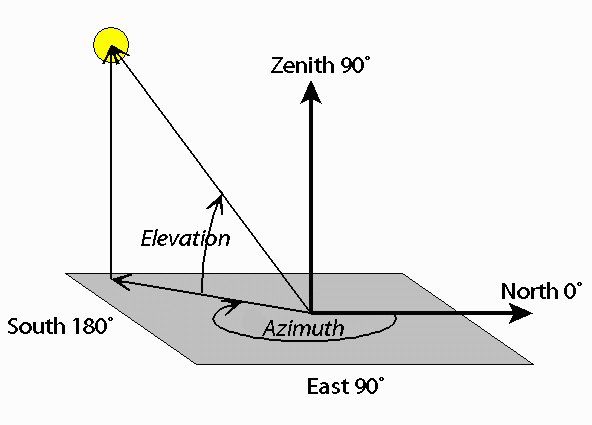
\includegraphics[width=0.4\textwidth]{az_elevation}
    \caption{Azimuthal and Elevation Visualization \cite{site-azElevationVisual}}
    \label{fig:az_elevation}
  \end{figure}

\subsection{GPS}\label{sec:components_gps}
A GPS should be selected for the ground station, and possibly for the PQ unit. In order to cater for Phase 2, and for simplified system development, a GPS module will be chosen that is suitable for both the PQ unit and the GS. To estimate GPS accuracy, a 1 degree variation is used (since the beamwidth of a typical antenna is an order of magnitude larger). A distance of \SI{100}{km} therefore results in a required accuracy of $2 \times 100 000 \times \pi \times \frac{1}{360} \approx \SI{2}{km}$, which is very large.

The NEO line of GPS modules from \textit{u-blox} are very commonly used, and are quoted to have a 2.5 m accuracy, however there was limited availability of these modules from local supplies (e.g. the \textit{NEO-6M}). Modules with similiar specifications from \textit{Makerbase} were therefore considered, such as the \textit{ATGM336H} and the \textit{ATGM332D}. Since both of these advertise 2.5 m accuracy, active antenna support, and current consumption less than 100 mA, the ATGM332D-5N31 was chosen for its lower price.

\subsection{IMU}
Generally, the ground station's orientation can be described by azimuthal and elevation angles as in Figure \ref{fig:az_elevation}. The ground station requires absolute azimuth angle measurement data, as well as elevation angle/tilt data, in order to orientate itself with respect to its surroundings. To determine absolute azimuthal rotation, the ground station should either be manually positioned to face north, or a magnetometer can be used. An accelerometer can be used to determine tilt rotation.

The above sensors, as well as a gyroscope, are typically packaged into an \textit{intertial measurement unit} (IMU). As seen in Section \ref{sec:components_gps}, only very primitive, low accuracy is required. \textit{Sensor fusion} is the mathematical process of converting raw sensor data into meaningful orientation angles. This is critical for fast-moving systems, where the accelerometer suffers during fast movements, and the gyroscope suffers due to noise drift over time.

The \textit{BNO055} is a 9-axis IMU which integrates an ARM Cortex-M0 to perform sensor fusion. It operates at 100 Hz, has $\SI{0.3}{\micro T}$ magnetic field resolution, and around 16 bit sensors. It, however, is very expensive (around R800). The \textit{MPU-9250}, and the \textit{MPU} line of IMU's in general, are seen as cheaper alternatives. Since the grouond station will be moving slowly, there is low requirement for complex sensor fusion algorithms. Since the MPU also has a 16-bit accelerometer, and only slightly lower magnetic field accuracy (\SI{0.6}{\micro T}), but is only around R150, it was selected.

\subsection{RF Communication}
The transciever for both the custom and proprietary protocol needs to be considered. There are a few options in this regard, from more to less specialized:
\begin{itemize}
    \item Fully custom design. Here, all components are discretely designed using transistors, MCUs etc.
    \item Front-End Module (FEM). For this option, the FEM provides filters, a low-noise amplifier (LNA), antenna matching, and down-conversion. Then, a controller (e.g. FPGA or MCU) needs to be designed to perform modulation/demodulation functionality (the \textit{modem}) and interface with the FEM.
    \item Dedicated Transciever. A transciever provides both the FEM functionality and the software modulation, however still requires RF techniques for matching, as well as an additional RF shield.
    \item Dedicated module. For this option, all functionality is provided in a dedicated modulate with an antenna and MCU interface. This is the easiest, but has little flexibility (e.g. since all matching is done internally, the frequency band is constrained).
    \item Software-defined radio. This is the most general option which are extremely general-purpose, but do not exercise the highest performance. They often can be connected to a computer via USB.
\end{itemize}

\subsubsection{Custom Communication}
For the custom protocol, a dedicated RF module will be used. It is ideal to experiment with LoRa, whilst having GFSK as a fallback. Fortunately, many LoRa modules also offer GFSK as a secondary modulation technique. Table \ref{tab:rfTransceivers} contrasts the two most common modules in the 433 MHz LoRa band which offer this feature. Most modules available are based on \textit{Semtech} chipsets due to the company's patent on the technology, and so there is little variation in performance. The RA-02 was ultimately selected due to its availability and cost.

\begin{table}[!htb]
  \centering
  \renewcommand{\arraystretch}{1.2}
  \begin{tabular}{ |c|c|c|c| }
  \hline
  \textbf{Name}   & \textbf{RX Sensitivity} & \textbf{TX Sensitivity}& \textbf{Frequency} \\
  \hline
  RA-02           & -141 dBm             & +17 dBm              & 410 to 525 MHz     \\
  RFM98           & -148 dBm             & +20 dBm              & 410 to 525 MHz     \\
  \hline
  \end{tabular}
  \caption{}
  \label{tab:rfTransceivers}
\end{table}

\subsubsection{Proprietary Communication}
Since the proprietary communication protocol will require reverse-engineering, and the exact encoding and GFSK parameters are unknown, SDR will be utilized to allow for flexibility. Universal Radio Hacker (URH) (https://github.com/jopohl/urh) is software available to investigate wireless protocols using an SDR. For this development, an easy-to-use USB SDR can be employed to investigate the protocol. The “RTLSDR” is considered the standard, low-cost solution for this.

\subsection{Stepper Motor Driver}
The original PCB of the previous antenna mount system contained two A3972 ICs to drive the stepper motors. Although these could be de-soldered and used, it is favourable to use a newer supported IC with better capabilities, and in case of damage. From the driver and motor datasheets, the following specifications are realized:
\begin{itemize}
    \item Dual DMOS Full-Bridge Output Configuration
    \item Bipolar PWM current control
    \item Micro-stepping (for smoother stepping)
    \item 0.5A, 24V
\end{itemize}

Very few drivers fit these exact specifications. The \textit{A4970} is considered the follow-up version of the \textit{A3972}, however is not available in a single pack. The L6219 driver is found to match these specifications and is readily available from a local supplier, and so will be selected.

\subsection{Power Distribution}
Both a 3.3V regulator and 5V regulator will be needed for the ground station power distribution. For this, the LD1117V33C and L7805CP will be used due to availability. A boost converter will also be needed to achieve the 24V motor drive voltage. A breakout board based on the XL6009 IC will be used from a local supplier.

\subsection{Microcontroller}
As discussed later, a general-purpose MCU will be needed both on the GS and the PQ. The three most popular frameworks/MCU types for this the ESP32, Arduino, and STM32.

The \textit{ESP32-WROOM-32} is a commonly available ESP32 variant which has 32 GPIO pins, of which several can be used as an ADC input, SPI or I2C interface. This means that there are 23x GPIO available, enough for this project. Further, the ESP32 has the added benefit of WiFi and Bluetooth connectivity, which may allow “smart” features to be added to either devices in the future. The \textit{ATMEGA328PB} is an MCU commonly used in small Arduino boards. It, however, has fewer pins than the ESP, and is also an 8-bit MCU, as opposed to the 32-bit ESP. It does, however, allow a supply  voltage of as low as 1.8V. Finally, the common \textit{STM32F411} MCU is a high-performance, ARM-Cortex board with highly accurate ADCs, up to 81 GPIOs, and a fast internal FPU.

Since the processing requirements for this project are not very high, and the ESP32 is a relatively high-performance MCU which satisfies the pin requirements and has added smart capabilities, it will be selected for the GS. For the PQ unit, an ATMEGA328PB will be used, due to its exceptionally low current consumption, and many fewer pins being needed for the PQ unit.